\input sys/inputs.tex
\usepackage[slovak]{babel}

\begin{document}

\bigheading{Plagáty v KSP}

% \info{task_name}{infile}{outfile}{points}{timelimit}{memlimit}
% leave this values, if you are not interested
\info{posters}{stdin}{stdout}{100}{2000 ms}{1 GB}

V tajnej základni Kamarátov Stratených Postulátov sa nachádza Stena. Na Stene
visia plagáty s prísne stráženými a hlavne nebezpečnými tajomstvami vesmíru.
Aby sa predišlo katastrofám a nechceným následkom, plagáty sa neprekrývajú
(môžu sa však dotýkať).

Raz za čas dojde nová várka plagátov hodných zavesenia na Stene. Kamaráti sa
pri takej vzácnej príležitosti stretávajú s obzvlášť ťažkým a závažným problémom:
Kam zavesiť nové plagáty? Našťastie majú zabehaný postup, ktorým sa riadia. Nanešťastie
je tento postup prenáramne komplikovaný. Vašou úlohou bude pomôcť s jedným krokom
tohto postupu.

Momentálne sa pre nové plagáty vyberajú sľubné pozície. Pre veľa pozícií rôznych
plagátov rýchlo spočítajte plochu pôvodných plagátov, ktorá by bola zakrytá
daným umiestnením nového plagátu.

\heading{Úloha}

Dostanete popis $n$ neprekrývajúcich sa šedých obdĺžnikov v bielej rovine. Ďalej dostanete $q$
dotazov na spracovanie v tvare: Aký je obsah šedej plochy v zadanom obdĺžniku? Pozor,
týmto \textbf{nepridávame} nový obdĺžnik do plochy.

Odpoveď spracujte online.

\heading{Vstup}

V prvom riadku dostanete päť čísel $r, c, n, q, m$, ($1 \leq r, c < m \leq 10^9 + 9$, $0 \leq n,q \leq 50\,000$),
šírku a výšku Steny, počet plagátov na stene, počet dotazov a špeciálny modulus
na počítanie dotazov (tento vysvetlíme ďalej).

Na každom z nasledujúcich $n$ riadkov budú štyri čísla, $x_1, y_1, x_2, y_2$ ($0 \leq x_1, x_2 \leq r$,
$0 \leq y_1, y_2 \leq c$), súradnice dvoch protiľahlých bodov obdĺžnika.

Nasleduje $q$ riadkov, v každom päť čísel $x_1^*, y_1^*, x_2^*, y_2^*, v$ v rozsahu od
$0$ po $m - 1$ vrátane. Z týchto čísel vypočítate reálne súradnice $x_1, y_1, x_2, y_2$
dotazovaného obdĺžnika pomocou vzorca dole.

Označme $l$ ako odpoveď na predošlý dotaz (pre úplne prvý dotaz položíme $l=0$). Potom
$$x_i = (x_i^* + l \cdot v) \pmod m$$
$$y_i = (y_i^* + l \cdot v) \pmod m$$

Dekódované súradnice $x_1, y_1, x_2, y_2$ spĺňajú nasledujúce podmienky:
$0 \leq x_1, x_2 \leq r$, $0 \leq y_1, y_2 \leq c$. 

\heading{Výstup}

Pre každý dotaz vypíšte jeden riadok obsahujúci jediné číslo: Odpoveď na dotaz.

\heading{Podúlohy}

Je viacero podúloh. V offline podúlohách bude hodnota $v$ vždy nulová.

\bigskip

\begin{center}
\begin{tabular}{|l|l|l|l|l|l|}
\hline
podúloha& body   & maximálne $r$& maximálne $c$ & maximálne $n$ a $q$ & online    \\ \hline
1       & 10     & $500$        & $500$         & $500$     & nie        \\ \hline
2       & 10     & $5000$       & $5000$        & $5000$    & nie        \\ \hline
3       & 40     & $300\,000$   & $300\,000$    & $50\,000$ & nie        \\ \hline
4       & 10     & $10^9$       & $200\,000$    & $50\,000$ & nie        \\ \hline
5       & 10     & $10^9$       & $10^9$        & $50\,000$ & nie        \\ \hline
6       & 10     & $100\,002$   & $100\,002$    & $50\,000$ & ano       \\ \hline
7       & 10     & $10^9 + 8$   & $10^9 + 8$    & $50\,000$ & ano       \\ \hline
\end{tabular}
\end{center}

\heading{Príklad}


\sampleIN
8 11 3 4 13
1 1 5 5
7 7 5 4
4 6 2 7
1 1 7 8 0
2 2 4 3 0
3 4 6 7 0
2 9 3 10 0
\sampleOUT
24
2
6
0
\sampleCOMMENT
Celú situáciu si môžete pozrieť na obrázku dole.
\sampleEND
\center{
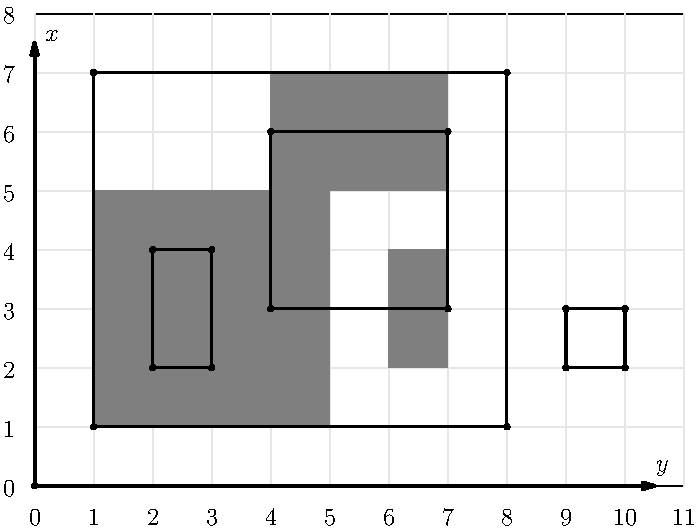
\includegraphics[width=12cm]{img/posters.pdf}
}

\sampleIN
8 11 3 4 13
1 1 5 5
7 7 5 4
4 6 2 7
1 1 7 8 4
6 6 8 7 2
2 3 5 6 7
11 5 12 6 5
\sampleOUT
24
2
6
0
\sampleCOMMENT
Toto je ten istý vstup ako prvý, ale využíva online dotazy.
\sampleEND
\end{document}
